% mainfile: ../RobertoDiRemigioPhDThesis.tex
\chapter{Continuum solvation models}\label{ch:CSM}


\begin{itemize}
    \item why and how continuum solvation models
    \item derivation of \acs{IEF}-\acs{PCM}, importance of Green's
      functions.
    \item \ac{BEM} and wavelet \acs{BEM} I think it's necessary to
      mention also ddCOSMO and ddPCM as alternative strategies (put a
      reference)
    \item variational formulation (no derivations, just mention the
      relevant literature)
\end{itemize}

\pagebreak

\section{Boundary integral equations}\label{sec:BIE}

\subsection{Transmission problem}
We assume Euclidean space $\mathbb{R}^3$ to be partitioned into two
subdomains $\Omegai$ and $\Omegae$ sharing a boundary $\Gamma$.
We further assume that $\Omegai$ is a closed domain, entirely contained inside $\Omegae$.
The transmission problem is posed as follows:
\todo[inline]{Some consideration on suitable functional spaces and the metric thereof.}
\begin{subequations}\label{eq:transmission}
\begin{align}
  \Li u &= f_\mathrm{i} \,\, \text{in}\,\, \Omegai \label{eq:internal} \\
  \Le u &= f_\mathrm{e} \,\, \text{in}\,\, \Omegae \label{eq:external} \\
  [u] &= \ue - \ui = g_\mathrm{D} \,\, \text{on}\,\, \Gamma
  \label{eq:trace-jump} \\
[\partial_L u] &= \partiale u - \partiali u = g_\mathrm{N} \,\,
\text{on}\,\, \Gamma \label{eq:conormal-jump} \\
|u| &\leq C \|x \|^{-1} \,\,\text{for}\,\,\| x \|\rightarrow\infty
\label{eq:radiation}
\end{align}
\end{subequations}
where the jump conditions (eqs. \eqref{eq:trace-jump} and
\eqref{eq:conormal-jump}) are given in terms of Dirichlet and Neumann
data for the solution $u$. The jump conditions are expressed in terms of
trace operators for the solution $u$ and its conormal derivative. For
notational simplicity, will use the symbols $\partiale$ and $\partiali$
for the latter and only give it in explicit form when needed. Please
refer to the book by \citeauthor{Sauter2011} for further details. The
fundamental solutions, or Green's functions, for the elliptic
differential operators $\Li$ and $\Le$ will be denoted by $\Gi$ and
$\Ge$, respectively.

\subsection{Boundary integral operators}
We introduce the relevant boundary integral operators for the abovementioned
transmission problem. They are three of the four components of the Calder\'on projector.
For $v \in L^2(\Gamma)$, $x, y \in \Gamma$:\footnote{We can assume a less restrictive functional space, \ie a Sobolev space of fractional order.}
\begin{equation}
\begin{aligned}
(\bi{S}_\star v)(x) &= \int_\Gamma G_\star(x, y)v(y)\diff y \\
(\bi{D}_\star v)(x) &= \int_\Gamma \partial_{L_\star,y}G_\star(x, y)v(y)\diff y \\
(\bi{D}^\dagger_\star v)(x) &= \int_\Gamma \partial_{L_\star,x}G_\star(x, y)v(y)\diff y \\
\end{aligned}
\end{equation}
where $\star$ is a placeholder for the $\mathrm{i}$ or $\mathrm{e}$ subscript.

\begin{lemma}[Properties of the boundary integral operators]
  The integral operators introduced above enjoy the following
  properties~\autocite{Hsiao2008, Sauter2011}:
  \begin{enumerate}
      \item on $L^2(\Gamma)$ $\bi{S}_\star$ is self-adjoint,
        $\bi{D}^\dagger_\star$ is the adjoint operator of
        $\bi{D}_\star$.
      \item The commutation relations:
        \begin{alignat}{2}
          \bi{D}_\star\bi{S}_\star = \bi{S}_\star\bi{D}^\dagger_\star, \quad&
          \bi{S}_\star\bi{D}_\star = \bi{D}^\dagger_\star\bi{S}_\star
        \end{alignat}
        hold
      \item The operators:
        \begin{subequations}
          \begin{align}
   \bi{S}_\star &: H^{-\frac{1}{2}}(\Gamma) \rightarrow H^{\frac{1}{2}}(\Gamma) \\
   \bi{D}_\star &: H^{\frac{1}{2}}(\Gamma) \rightarrow H^{\frac{1}{2}}(\Gamma) \\
   \bi{D}^\dagger_\star &: H^{-\frac{1}{2}}(\Gamma) \rightarrow H^{-\frac{1}{2}}(\Gamma)
          \end{align}
        \end{subequations}
      \item The operator $\bi{S}_\star$ is coervice and admits a
        continuous inverse in the aforementioned Sobolev spaces.
      \item The operators $\lambda - \bi{D}_\star$ and $\lambda -
        \bi{D}^\dagger_\star$ with $\lambda \in (-2\pi, +\infty)$
        admit a continuous inverse in the aforementioned
        Sobolev spaces.
  \end{enumerate}
\end{lemma}

\subsection{Lemma of Integral Representation}
For the transmission problem \ref{eq:transmission} there holds:
\begin{itemize}
\item $\forall x \in \Omegai$
\begin{equation}
u = \bi{S}_\mathrm{i}(\partiali u)
- \bi{D}_\mathrm{i}(\ui) + \int_{\Omegai} \Gi f_\mathrm{i}\diff y
\end{equation}
\item $\forall x \in \Omegae$
\begin{equation}
u = -\bi{S}_\mathrm{e}(\partiale u)
+ \bi{D}_\mathrm{e}(\ue) + \int_{\Omegae}\Ge f_\mathrm{e}\diff y
\end{equation}
\item $\forall x \in \Gamma$
  \begin{equation}\label{eq:stat3}
    \frac{1}{2}\ui = \bi{S}_\mathrm{i}(\partiali u)
    - \bi{D}_\mathrm{i}(\ui) + \int_{\Omegai}\Gi f_\mathrm{i}\diff y
  \end{equation}
\item $\forall x \in \Gamma$
  \begin{equation}\label{eq:stat4}
    \frac{1}{2}\ue = -\bi{S}_\mathrm{e}(\partiale u)
    + \bi{D}_\mathrm{e}(\ue) + \int_{\Omegae}\Ge f_\mathrm{e}\diff y
  \end{equation}
\end{itemize}

\pagebreak
\section{IEFPCM}\label{sec:IEF}

Note that the figures refer to cases where the dielectric is supposed to
be homogeneous and isotropic. The derivation are, however, general and
do not assume homogeneity and isotropy.
The source charge densities are not assumed to be continuous, the
hypothesis that they are entirely supported in either of the internal or
external subdomains is however made:
\begin{alignat}{2}
  \Supp(\rhoi) \subseteq \Omegai, \quad& \Supp(\rhoe) \subseteq \Omegae
\end{alignat}

%%%% CASE 0

\subsection{Case 0: sources in a vacuum cavity inside a dielectric}

\begin{figure}[h!]
  \centering
  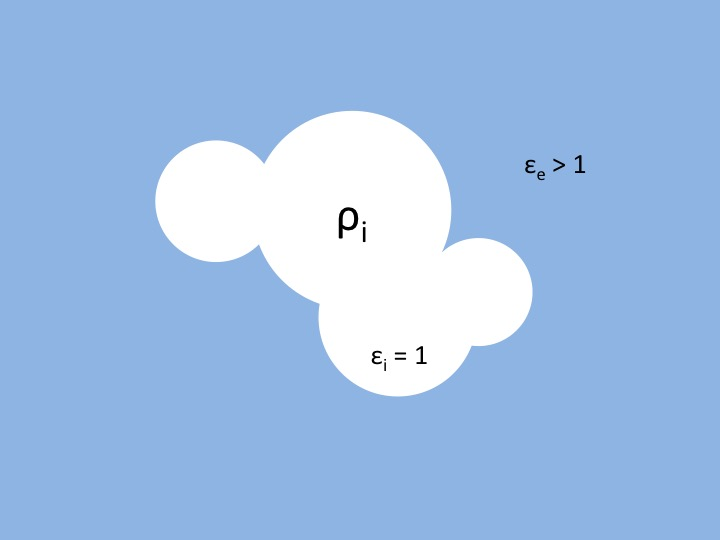
\includegraphics[width=.65\textwidth]{case0}
  \caption{Vacuum Cavity in dielectric with permittivity $\diel_\mathrm{e}>1$.
  Source charge density $\rho_\mathrm{i}$ inside the cavity
  ($\diel_\mathrm{i}=1$). \textcolor{red}{Regular IEF}}
  \label{fig:case0}
\end{figure}

This is the regular IEF as derived in:~\autocite{Cances1998}
\begin{subequations}
\begin{align}
  \nabla^2 u &= \rhoi \,\, \text{in}\,\, \Omegai \\
  \Le u &= 0 \,\, \text{in}\,\, \Omegae \\
  [u] &= \ue - \ui = 0 \,\, \text{on}\,\, \Gamma \\
[\partial_L u] &= \partiale u - \partiali u = 0 \,\,
\text{on}\,\, \Gamma \\
|u| &\leq C \|x \|^{-1} \,\,\text{for}\,\,\| x \|\rightarrow\infty
\end{align}
\end{subequations}

We introduce the following auxiliary potential:
\begin{equation}
  h(x) =
  \begin{cases}
    &\int_{\mathbb{R}^3}\Gi\rhoi(y)\diff y  \quad x \in \Omegai \\
    &\int_{\mathbb{R}^3}\Ge\rhoi(y)\diff y  \quad x \in \Omegae
  \end{cases}
\end{equation}
for which we have:\footnote{This can be checked by applying the
differential operators to the definition of $h$ and then swapping
differentiation and integration.}
\begin{equation}
  \begin{cases}
    \nabla^2 h &= \rhoi \,\, \text{in}\,\, \Omegai \\
    \Le h &= 0 \,\, \text{in}\,\, \Omegae
  \end{cases}
\end{equation}
We then define the \emph{reaction potential} as:
\begin{equation}
  \xi = u - h
\end{equation}
such that:
\begin{subequations}
\begin{align}
  \nabla^2 \xi &= 0 \,\, \text{in}\,\, \Omegai \\
  \Le \xi &= 0 \,\, \text{in}\,\, \Omegae \\
  -[\xi] &= [h] \,\, \text{on}\,\, \Gamma \\
  -[\partial_L \xi] &= [\partial_L h] \,\, \text{on}\,\, \Gamma
\end{align}
\end{subequations}
inside the cavity, the reaction potential can be represented by a
\emph{single layer potential}, \ie by an apparent surface charge (ASC):
\begin{equation}
  \xi_\mathrm{i} = \bi{S}_\mathrm{i}\sigma
\end{equation}

Applying Eqs. \eqref{eq:stat3} and \eqref{eq:stat4} of the Lemma of Integral
Representation to the reaction potential yields:
\begin{align}
  \frac{1}{2}\xi_\mathrm{i} &= \bi{S}_\mathrm{i}(\partiali \xi) -
  \bi{D}_\mathrm{i}(\xi_\mathrm{i}) \\
  -\frac{1}{2}\xi_\mathrm{e} &= \bi{S}_\mathrm{e}(\partiale \xi) -
  \bi{D}_\mathrm{e}(\xi_\mathrm{e})
\end{align}
in both cases the last term, including the integration over the entire
subdomain volume, drops out ($f_\mathrm{i} = 0 = f_\mathrm{e}$).
While use of Eq. \eqref{eq:stat4} on the auxiliary potential $h$ yields:
\begin{equation}
  -\frac{1}{2}h_\mathrm{e} =
  \bi{S}_\mathrm{e}(\partiale h) -
  \bi{D}_\mathrm{e}(h_\mathrm{e})
\end{equation}
Together with the jump conditions one obtains:
\begin{subequations}
  \begin{align}
    &\bi{S}_\mathrm{i}(\partiali \xi) - \bi{D}_\mathrm{i}(\xi_\mathrm{i})
    = \frac{1}{2}\xi_\mathrm{i} \label{eq:first} \\
    &\bi{S}_\mathrm{e}(\partiale \xi) - \bi{D}_\mathrm{e}(\xi_\mathrm{e})
    = -\frac{1}{2}\xi_\mathrm{e} \label{eq:second} \\
  &\bi{S}_\mathrm{e}(\partiale h) - \bi{D}_\mathrm{e}(h_\mathrm{e})
  = -\frac{1}{2}h_\mathrm{e} \label{eq:third} \\
  &\xi_\mathrm{i} - \xi_\mathrm{e} = h_\mathrm{e} - h_\mathrm{i}
  \label{eq:fourth} \\
  &\partiali \xi - \partiale \xi = \partiale h - \partiali h
  \label{eq:fifth}
  \end{align}
\end{subequations}

\begin{enumerate}
  \item Add Eqs. \eqref{eq:second} and \eqref{eq:third}:
    \begin{equation}
    \bi{S}_\mathrm{e}(\partiale \xi + \partiale h) -
    \bi{D}_\mathrm{e}(\xi_\mathrm{e} + h_\mathrm{e})
    = -\frac{1}{2}(\xi_\mathrm{e} + h_\mathrm{e})
    \end{equation}
  \item Exploit Eqs. \eqref{eq:fourth} and \eqref{eq:fifth} to
    eliminate the external traces and conormal derivatives:
    \begin{equation}
      \bi{S}_\mathrm{e}(\partiali \xi) + \left(\frac{1}{2} -
      \bi{D}_\mathrm{e}\right)\xi_\mathrm{i} =
      - \bi{S}_\mathrm{e}(\partiali h) - \left(\frac{1}{2} -
      \bi{D}_\mathrm{e}\right)h_\mathrm{i}
    \end{equation}
  \item Introduce the integral representation of
    $\xi_\mathrm{i}$:
    \begin{equation}
      \bi{S}_\mathrm{e}(\partiali \xi) + \left(\frac{1}{2} -
      \bi{D}_\mathrm{e}\right)\bi{S}_\mathrm{i}\sigma =
      - \bi{S}_\mathrm{e}(\partiali h) - \left(\frac{1}{2} -
      \bi{D}_\mathrm{e}\right)h_\mathrm{i}
    \end{equation}
  \item Reorganize Eq. \eqref{eq:first}, using the commutation
    relation and the integral representation of $\xi_\mathrm{i}$:
    \begin{equation}
    \partiali \xi = \left(\frac{1}{2} + \bi{D}^\dagger_\mathrm{i}\right)\sigma
    \end{equation}
    such that:
    \begin{equation}
      \left[ \bi{S}_\mathrm{e}\left(\frac{1}{2} + \bi{D}^\dagger_\mathrm{i}\right)
      +
      \left(\frac{1}{2} - \bi{D}_\mathrm{e}\right)\bi{S}_\mathrm{i}
      \right]\sigma =
      - \bi{S}_\mathrm{e}(\partiali h) - \left(\frac{1}{2} -
      \bi{D}_\mathrm{e}\right)h_\mathrm{i}
    \end{equation}
  \item Employ the Dirichlet-to-Neumann (DtN) map to simplify
    the RHS. The DtN map is derived by applying Eq. \eqref{eq:stat3} to
    the Newton potential:
    \begin{equation}
      \phi(x) = (\bi{N}\rhoi)(x) = \int_{\mathbb{R}^3}\Gi\rhoi(y)\diff y
      = \left.h(x)\right|_{\Omegai}
    \end{equation}
    which is equal, in $\Omegai$, to the auxiliary potential $h(x)$.
    With this definition one has:
    \begin{equation}
      \frac{1}{2}\phi_\mathrm{i} =
      \bi{S}_\mathrm{i}(\partiali \phi) -
      \bi{D}_\mathrm{i}(\phi_\mathrm{i}) + \int_{\Omegai}\Gi\rhoi(y)\diff y
      =
      \bi{S}_\mathrm{i}(\partiali \phi) -
      \bi{D}_\mathrm{i}(\phi_\mathrm{i}) + \phi_\mathrm{i}
    \end{equation}
    eventually leading to the DtN map:
    \begin{equation}\label{eq:regular-DtN}
      \left(\frac{1}{2} - \bi{D}_\mathrm{i}\right)\phi_\mathrm{i}
      +\bi{S}_\mathrm{i}(\partiali \phi) = 0
    \end{equation}
  \item Having identified $\phi_\mathrm{i} \equiv h_\mathrm{i}$
    and $\partiali \phi \equiv \partiali h$ and employing the DtN map,
    Eq.\eqref{eq:regular-DtN}, one obtains the IEF-PCM equation:
    \begin{equation}\label{eq:regular-IEF}
      \left[ \bi{S}_\mathrm{e}\left(\frac{1}{2} + \bi{D}^\dagger_\mathrm{i}\right)
      +
      \left(\frac{1}{2} - \bi{D}_\mathrm{e}\right)\bi{S}_\mathrm{i}
      \right]\sigma =
      -\left[\left(\frac{1}{2}-\bi{D}_\mathrm{e}\right)
      -\bi{S}_\mathrm{e}\bi{S}_\mathrm{i}^{-1}
       \left(\frac{1}{2}-\bi{D}_\mathrm{i}\right)
      \right]\phi
    \end{equation}
    where the subscript $\mathrm{i}$ for the Newton potential $\phi$ has
    been dropped, given that it is continuous across the boundary
    $\Gamma$.
\end{enumerate}
The above proves the existence of a representation of the reaction
potential valid \emph{inside} the cavity in terms of an apparent surface
charge density. We do not prove the uniqueness of this solution and
refer the interested reader to the original paper.~\autocite{Cances1998}

In the code, the Green's functions are defined \emph{without} the $4\pi$
factors in the denominator. Instead of $\frac{1}{2}$ as coefficients to
the identity operator, one will then have $2\pi$:
\begin{equation}\label{eq:regular-IEF-2pi}
  \left[ \bi{S}_\mathrm{e}\left(2\pi + \bi{D}^\dagger_\mathrm{i}\right)
  +
  \left(2\pi - \bi{D}_\mathrm{e}\right)\bi{S}_\mathrm{i}
  \right]\sigma =
  -\left[\left(2\pi-\bi{D}_\mathrm{e}\right)
  -\bi{S}_\mathrm{e}\bi{S}_\mathrm{i}^{-1}
  \left(2\pi-\bi{D}_\mathrm{i}\right)
  \right]\phi
\end{equation}

\paragraph{Isotropic IEF}
From Eq. \eqref{eq:regular-IEF-2pi} we can derive the isotropic IEF,
the DPCM and the CPCM (by letting $\diel\rightarrow\infty$) equations.
For a homogeneous, isotropic dielectric with permittivity $\diel$ the
Green's function outside the cavity is simply given by scaling the one
inside:
\begin{equation}
  \Ge = \frac{1}{\diel|x-y|} = \frac{1}{\diel} \Gi = \frac{1}{|x-y|}
\end{equation}
leading to the boundary integral operators:
\begin{alignat}{2}
  \bi{S}_\mathrm{i} = \diel\bi{S}_\mathrm{e} = \bi{S}, \quad&
  \bi{D}_\mathrm{i} = \bi{D}_\mathrm{e} = \bi{D}
\end{alignat}
Eventually, one has:
\begin{equation}
  \left[ 2\pi \left(\frac{\diel+1}{\diel-1}\right)
  - \bi{D} \right]\bi{S}\sigma
  =
  -\left[2\pi-\bi{D}\right]\phi
\end{equation}

\section[Variational Formulation of Classical Polarizable Models]{
A Unifying View of Classical Polarizable Models within a Variational Formulation}
\label{sec:variational}

Variational functional for implicit models, \acs{PCM} in this case:
\begin{equation}
 U_\mathrm{PCM} = \frac{1}{2}\scalprod{\sigma}{\PCM\sigma} + \scalprod{\esp}{\sigma}
\end{equation}

Variational functional for explicit models, could be MMpol or PE or FQ:
\begin{equation}
  U_\mathrm{MM} = \frac{1}{2}\kappa\MM\kappa + \kappa\zeta
\end{equation}

The PCM equations will be written in the ``complete basis'' meaning that
we will introduce the usual boundary-element method (BEM) discretization
at the very end of the derivation. In other words, we will be working
with the exact integral equation and not with its discretized
counterpart. As a consequence, the apparent surface charge $\sigma$ and
the electrostatic potential $\esp$ will have a \emph{continuous}
dependence on a ``cavity surface'' index $\vect{s}$. Whenever a
charge-potential product is present it is then to be interpreted as the
\emph{surface integral}, i.e. the scalar product in the suitable,
infinite-dimensional vector space on the cavity boundary $\Gamma$. The
following shorthand notation will be adopted:
\begin{equation}
 \sigma\esp = \scalprod{\sigma}{\esp}
\end{equation}

Coupled implicit/explicit polarization energy functional:
\begin{equation}\label{eq:pcm-mm-functional}
  U_\mathrm{pol} =
   \frac{1}{2}\sigma\PCM\sigma + \sigma\esp
 + \frac{1}{2}\kappa\MM\kappa + \kappa\zeta
 + \sigma\bi{X}\kappa
\end{equation}
where one has:
\begin{equation}
  \sigma\MMPCM\kappa = \kappa\MMPCM^\dagger\sigma
\end{equation}
and $\MMPCM$ is the implicit/explicit interaction kernel. This is
charge/dipole or charge/charge interaction kernel for the MMpol and PE models
or the FQ model, respectively.
The global minimum of the convex functional is found by differentiating
it with respect to the variational degrees of freedom, \ie{} the
\acl{ASC} (\acs{ASC}) density $\sigma$ and the classical point
charges/dipoles $\kappa$. This leads to the coupled equations:
\begin{align}
  \PCM\sigma + \esp + \MMPCM\kappa &= 0 \\
  \MM\kappa  + \zeta + \MMPCM^\dagger\sigma &= 0
\end{align}
or in the commonly found matrix form:
\begin{equation}
  \begin{pmatrix}
    \PCM & \MMPCM \\
    \MMPCM^\dagger & \MM
  \end{pmatrix}
  \begin{pmatrix}
   \sigma \\
   \kappa
  \end{pmatrix}
  =
  -
  \begin{pmatrix}
   \esp \\
   \zeta
  \end{pmatrix}
\end{equation}
Finally, let us re-express the equations above in a "supermatrix"
formalism:
\begin{equation}
  U_\mathrm{pol} =
  \frac{1}{2}{}^t\p\V\p + {}^t\p\s
\end{equation}
where:
\begin{alignat}{3}
  \p =
  \begin{pmatrix}
    \sigma \\
    \kappa
  \end{pmatrix},
  \quad&
  \s =
  \begin{pmatrix}
   \esp \\
   \zeta
  \end{pmatrix},
  \quad&
  \V =
  \begin{pmatrix}
    \PCM & \MMPCM \\
    \MMPCM^\dagger & \MM
  \end{pmatrix}
\end{alignat}
and the ${}^t\p$ symbol denotes the transposed supervector $\p$.
The supermatrix form will prove particularly useful in the following
derivations.

\todo[inline]{PUT REFERENCES HERE!!!}
The variational formulation offers a series of advantages.
The classical energy functional:
\begin{equation}
  U_\mathrm{pol} =
   \frac{1}{2}\sigma\PCM\sigma + \sigma\esp
 + \frac{1}{2}\kappa\MM\kappa + \kappa\zeta
 + \sigma\bi{X}\kappa
\end{equation}
renders itself to a straightforward physical interpretation. In the
three bilinear terms, \ie{} the ones mediated by an interaction
operator, we can identify the self-interaction of the classical
polarization with itself, be it purely implicit:
$\frac{1}{2}\sigma\PCM\sigma$, purely explicit
$\frac{1}{2}\kappa\MM\kappa$ or mixed $\sigma\MMPCM\kappa$.
These terms are positive definite and give rise to an unfavorable
contribution, which is counterbalanced by the linear terms. These terms
mediate the interaction between the induced polarization and the
inducing fields: $\esp$ and $\zeta$. While $\esp$ is quite clearly the
\acl{MEP} (\acs{MEP}), $\zeta$ can either be the molecular electric
field (MMpol and PE models) or again the \acs{MEP} (FQ model).
In any case, both will be determined by the quantum mechanical molecular
charge density and can thus be formulated as expectation values of
one-electron operators. Eventually, this achieves the coupling between
the classical -- $\sigma$ and $\kappa$ -- and
the quantum mechanical variational degrees of freedom.

\todo[inline]{Mention the classical equivalent of the Hellmann--Feynman
theorem and why it is particularly useful in formulating response
theory.}
